After outlining goals and preconditions in the previous section, this section
presents the architecture of the KVS. It covers all aspects, except crash
consistency and concurrency control which are dealt with in more detail in
subsequent sections.

The KVS is designed for multi-core architectures and relies on both volatile and
non-volatile memory attached to the system memory interface. In order to take
advantage of both types of memory, the KVS is designed as a two-level store
which only updates NVRAM when a transaction commits. Consistency across crashes
is ensured with existing hardware primitives and upcoming platform features.
Concurrent transactions are controlled by a serializable variant of SI.
Background on these design decisions is given below.

\subsection{System Architecture}

Designing a runtime-critical software such as databases not only involves
knowledge about expected workloads but also about the underlying computing
device. While workloads have been discussed earlier, this section describes the
system architecture of the intended KVS.

\subsubsection{Concurrency}

The KVS is designed for a single-node architecture. Even though distributed
databases are fairly common, there seems to be no apparent reason for them to
reveal any more insight on leveraging NVRAM for concurrency. Also distributed
systems involve much more complex mechanisms such as consensus among distributed
transactions, all of which are beyond the scope of this work. However, future
work should investigate whether the conclusions of this work also hold for
distributed databases.

In order to achieve scalable transaction throughput through concurrency, the
target system is a multi-core architecture. That means, the system features one
or more processors with multiple cores, where each core may support multiple
hardware threads. On such a system, each transaction is executed in the context
of a thread which is scheduled and assigned to a processor core by the operating
system. Processors usually coordinate their work by communicating via some form
of chip interconnect. In order to preserve generality, this work makes no
assumptions concerning the nature of such interconnect networks.

\begin{figure}[!ht]
    \centering
    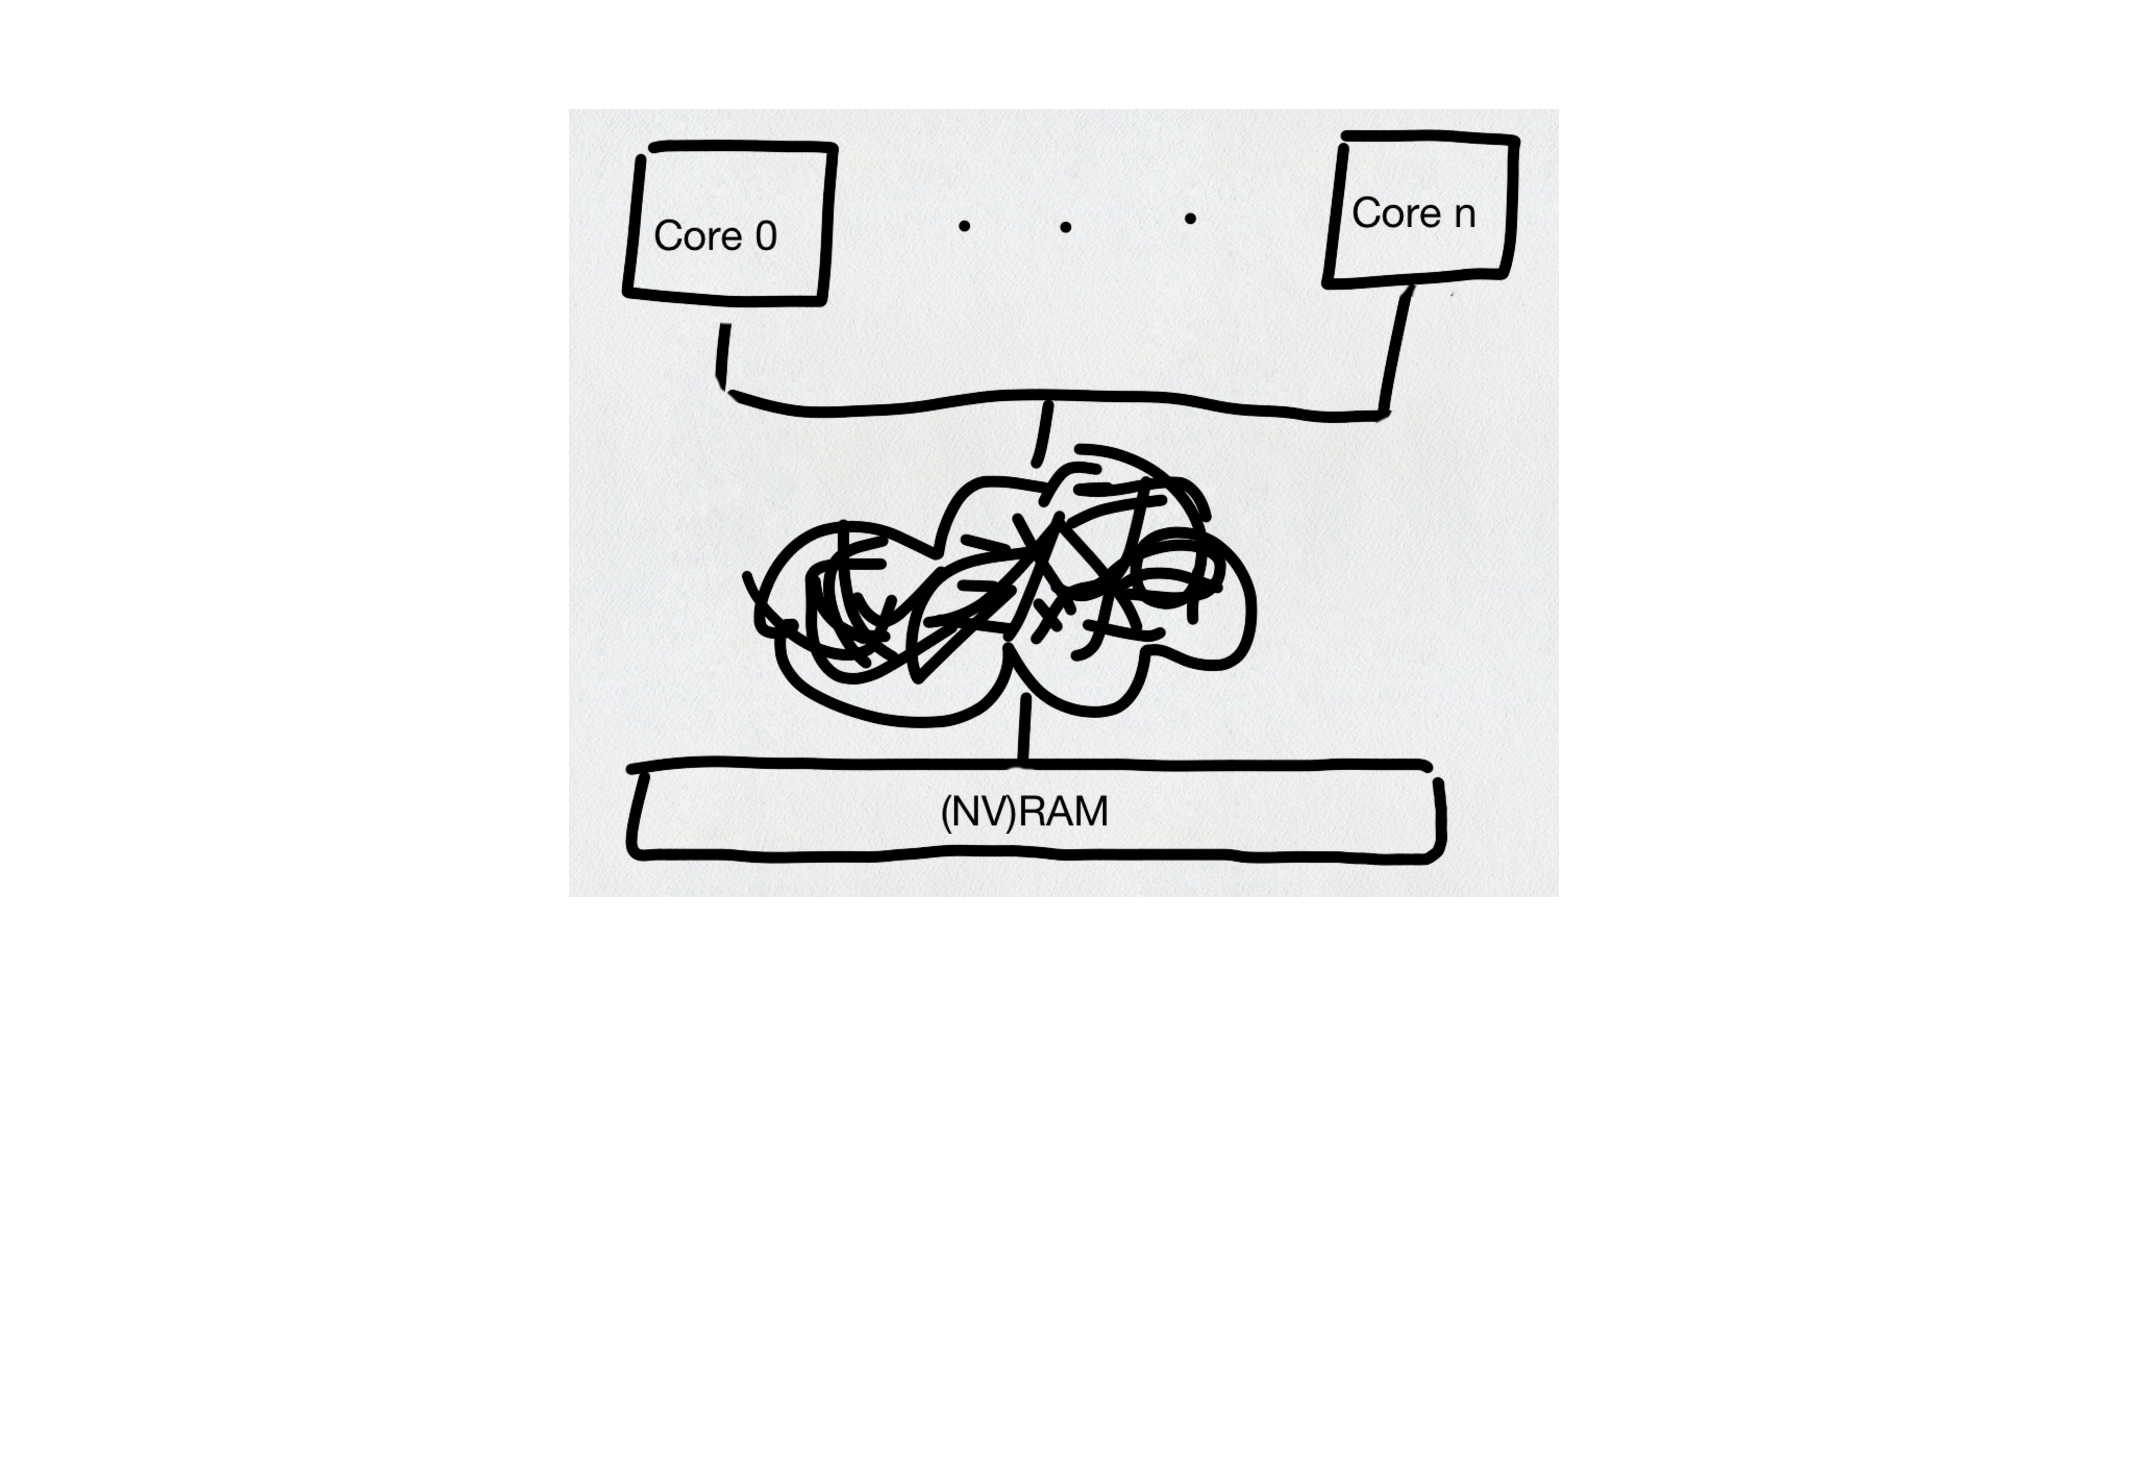
\includegraphics[scale=0.5]{figures/drafts/concept-sys-cpu.pdf}
    \caption{}
    \label{fig:concept-sys-cpu}
\end{figure}

\subsubsection{Memory Architecture}

Recent research shows that on traditional hardware it is advisable to continue
integrating volatile RAM together with NVRAM. The reason is that not all data is
meant to be durable which is especially true for NVRAM where crash consistency
is linked with considerable overhead. Manufacturing NVRAM is still challenging,
especially in terms of access latency and endurance, but it is expected that
these issues will be resolved in the near future. Therefore, in an effort to
combine the benefits of both technologies, the memory subsystem is required to
feature both volatile RAM and NVRAM. In accordance with recent research it is
assumed that both kinds of memory can be accessed through the same memory
interface. This work assumes a shared memory architecture. That is, processors
may have one or more private cache levels but main memory is accessible to all
processors. Conceptually, cache coherence is not required but has the advantage
that less effort is spent on coordinating concurrent access to shared data.

The KVS is designed to exclusively reside in main memory. All data that is not
required across restarts is stored in volatile RAM, whereas all other data are
stored in NVRAM. Multiple recent works have demonstrated that NVRAM can be used
to build MMDB without conventional non-volatile storage such as hard drives. As
a result, ensuring recovery, which has always been an inherent bottleneck of
MMDB, can be eliminated. In addition, near-instantaneous restarts become
feasible. As a consequence, conventional storage is not part of the concept for
this KVS. While such components may very well be present in a system, they are
never used to store any data of the KVS other than its binaries. This way, data
access incurs no I/O and restarts do not have to fetch data from slower storage
devices. In return, candidate systems must provide sufficient NVRAM capacity to
hold the entire database.

\begin{figure}[!ht]
    \centering
    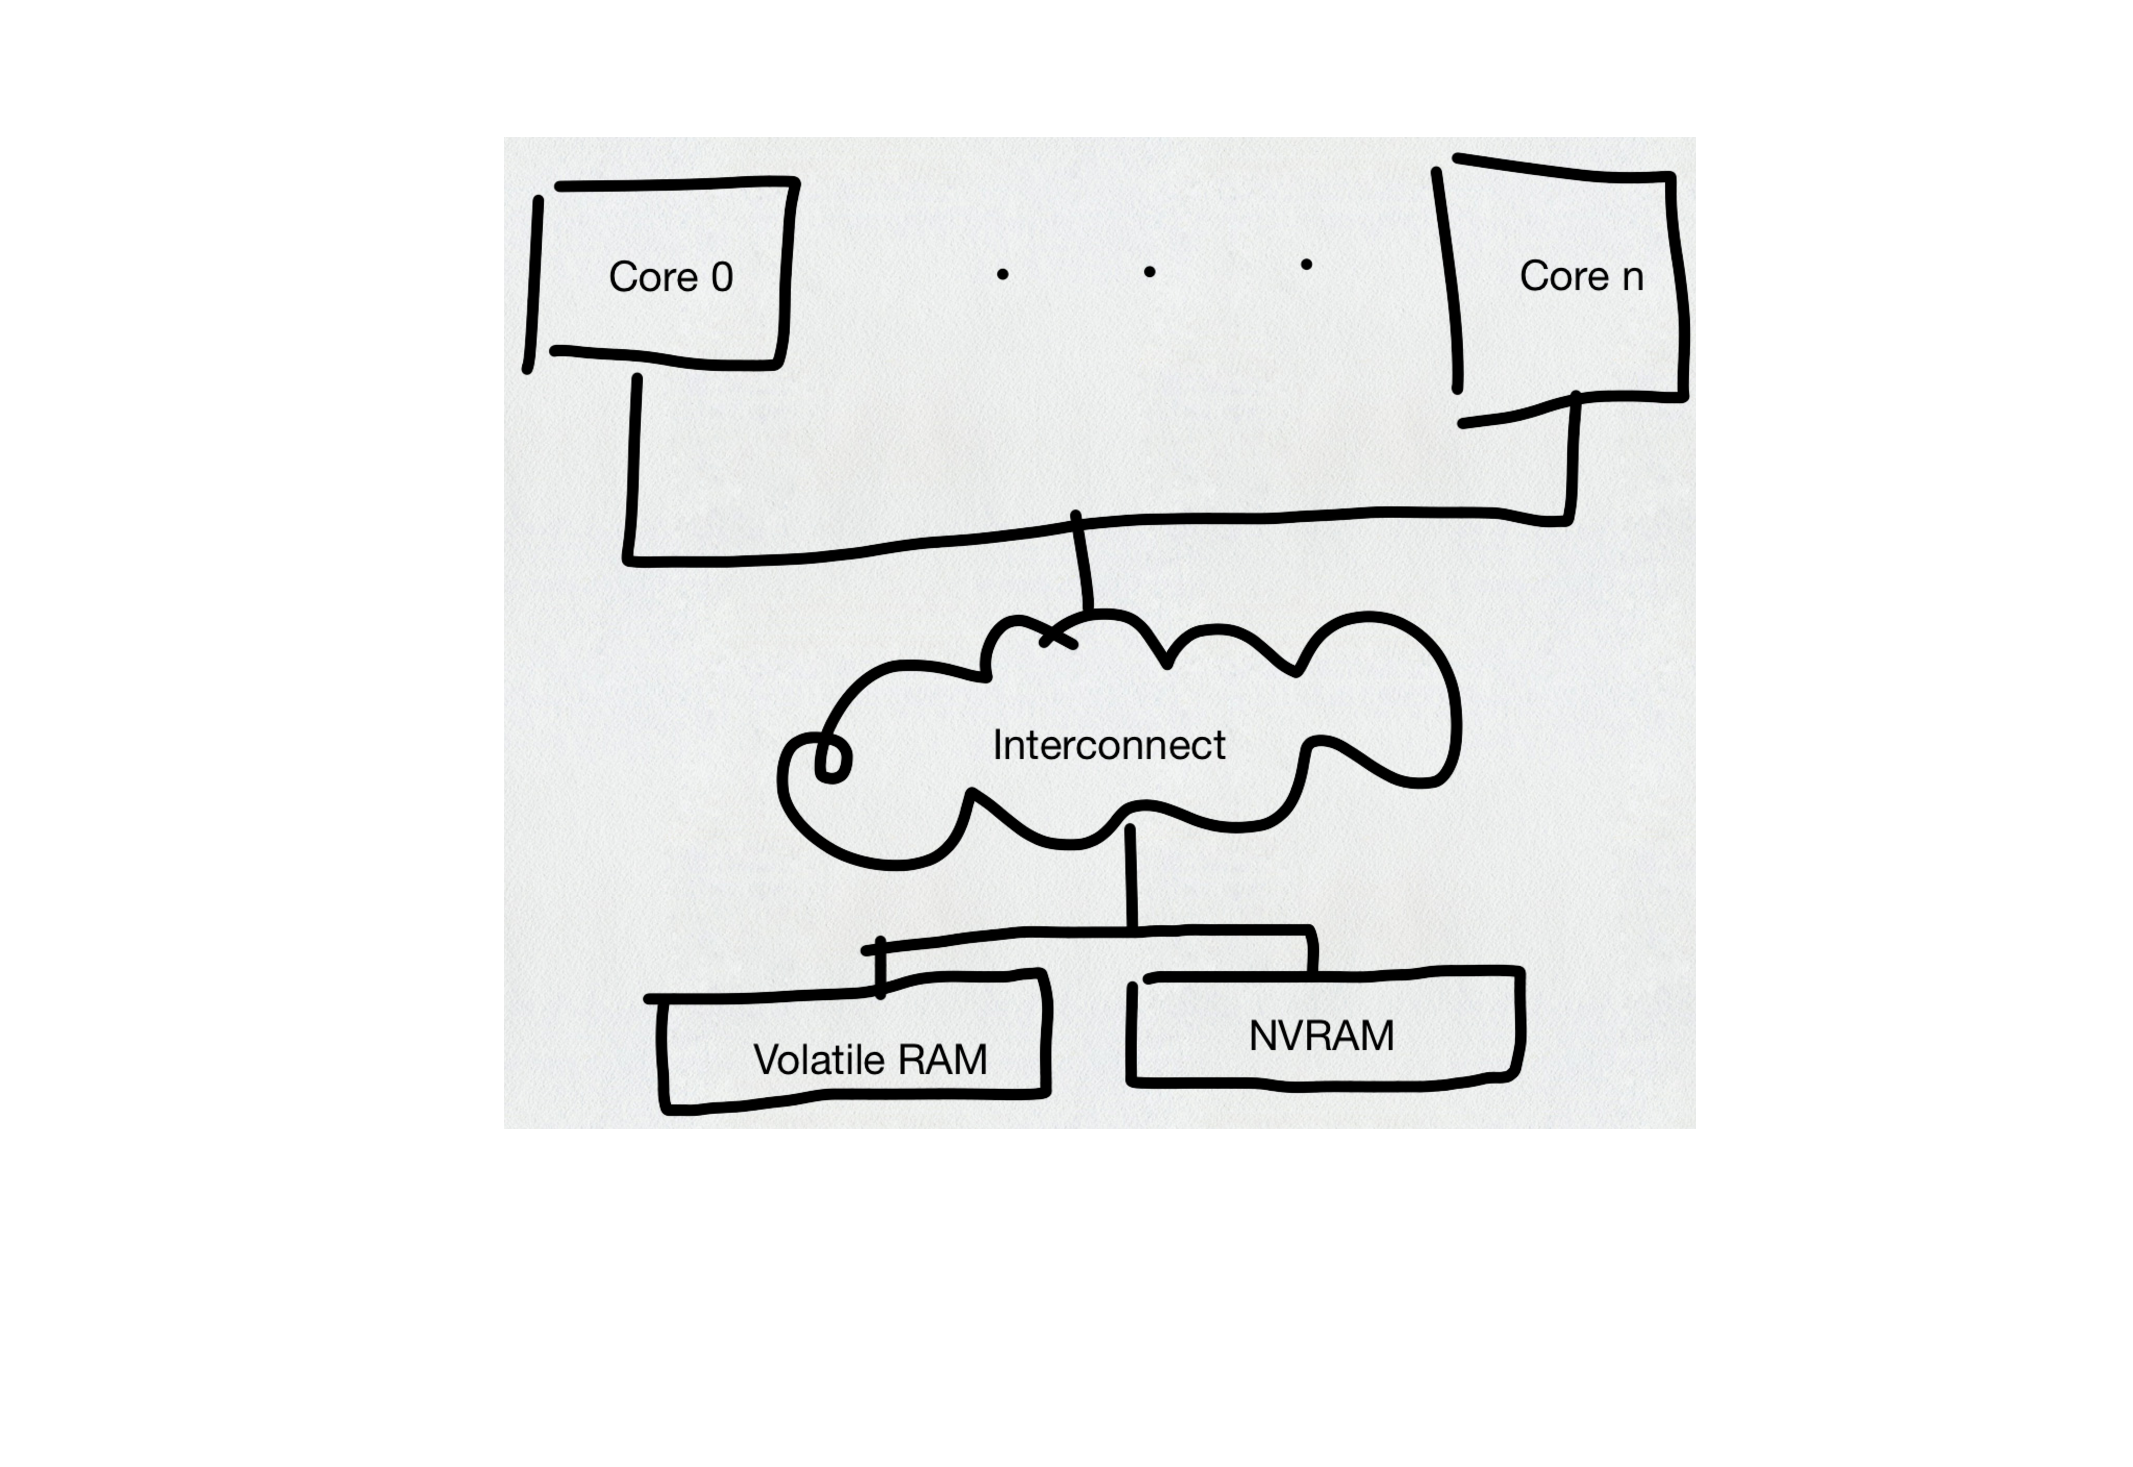
\includegraphics[scale=0.5]{figures/drafts/concept-sys-mem.pdf}
    \caption{}
    \label{fig:concept-sys-mem}
\end{figure}

A disadvantage of this approach is that the size of the database is bounded by
the amount of available NVRAM. In contrast, MMDB usually allow for larger data
sets by keeping frequently used data in memory, while others are moved to slower
mass storage media. However, main memory capacities have been steadily growing
and NVRAM capacities are projected to have at least twice the capacity of DRAM.
Another drawback is recoverability in case of device failures. Mass storage not
only scales better in terms of capacity, but it also supports redundancy through
RAID, for instance. With NVRAM, both capacity and scalability are lower, so
employing information redundancy may be prohibitively expensive. Without such
measures of fault tolerance, however, a single failed NVRAM module may lead to
permanent data loss. This issue is not tackled in this thesis and is therefore
left for future work.

\subsection{Key-Value Store Design}

This section describes the software architecture of the KVS. That includes the
operation principle in terms of transactions, storage, and concurrency as well
as the general structure.

\subsubsection{Two-Level Store}

As mentioned above, the KVS resides entirely in main memory. This enables fast
access to all data within the database and makes swapping obsolete. In return,
the size of the database is bounded by the total NVRAM capacity. Apart from
capacity, operating NVRAM currently exhibits greater access latencies compared
to DRAM. As pointed out in Chapter \ref{ch:nvram}, these latencies mainly affect
writes and are attributed to both technology parameters and crash consistency
measures. This work assumes, that even as technology improves, crash consistency
will continue to come a cost.

In an effort to mitigate these issues, the KVS is designed to use volatile RAM
in addition to NVRAM. In order to achieve maximum performance, it attempts to
exploit the benefits of either technology while limiting the impact of their
drawbacks. For that purpose, the KVS employs a two-level store architecture as
in \cite{bailey2013exploring}.

In a two-level store architecture, in-flight data from memory accesses may be
buffered in an intermediary storage medium. In this case, write operations are
buffered in volatile memory until their associated transaction commits. Only
when a transaction commits, all its updates are propagated to NVRAM. Otherwise,
no user data is written to NVRAM. Read operations are not directly affected by
the two-level store paradigm. In some cases, however, an implementation may
choose to buffer read operations, for instance to determine serialization order.

The aim of the two-level store architecture is to reduce the impact of
NVRAM-related latencies. Buffering updates to NVRAM in volatile memory has
several advantages. First, updates are only posted to NVRAM when they need to
be which can save both latency and memory bandwidth, especially when aborts are
frequent. Second, limiting updates to NVRAM to commit phases allows for bulk
writes. This way, expensive consistency procedures do not have to be performed
repeatedly for a single transaction. Third, updated items in volatile memory can
be accessed with lower latencies, which is true for both read and write
operations. In the end, buffering updates also aids recovery, as uncommitted
data is guaranteed to be lost after a restart.

\begin{figure}[!ht]
    \centering
    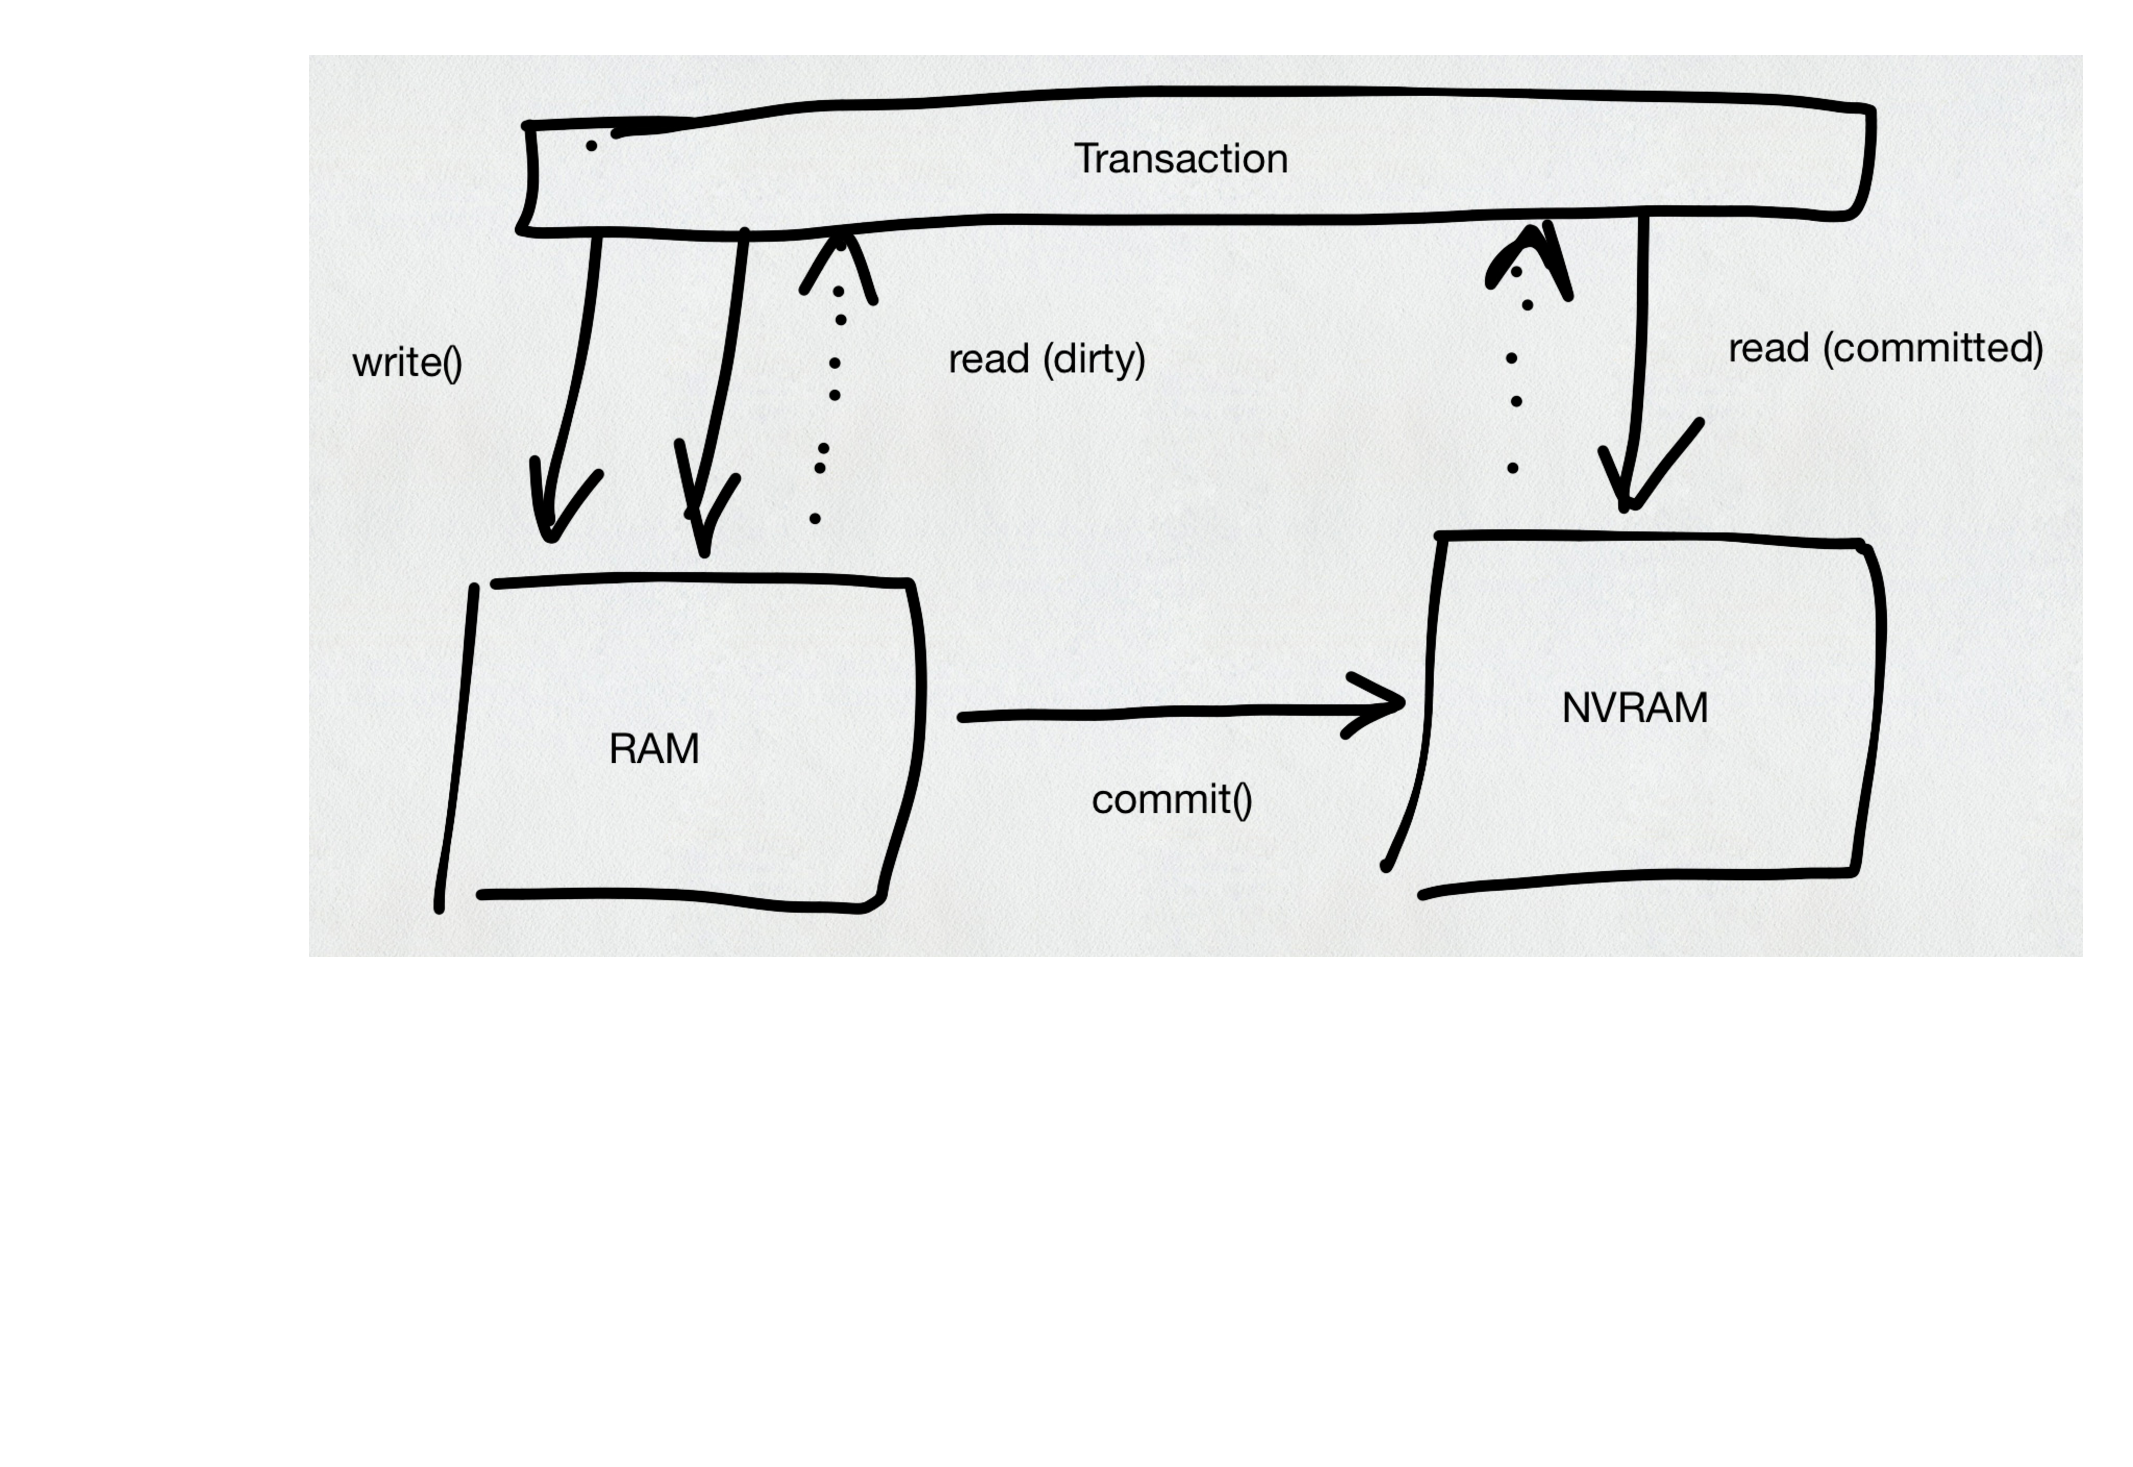
\includegraphics[width=\textwidth]{figures/drafts/concept-sys-two-level-store.pdf}
    \caption{}
    \label{fig:concept-two-level-store}
\end{figure}

\subsubsection{Transactions}

The KVS supports full-featured and ACID-compliant transactions. Unlike other
works, this KVS allows multiple operations to be enclosed in a single
transaction. The primary motivation behind this decision is to preserve
generality with regard to more complex DBMS. Likewise, all transactions must
conform to the ACID properties to ensure data consistency. Nesting transactions
is not supported as use cases are too few to justify the additional complexity.

Providing ACID support requires a conjunction of preventing erroneous behaviour
and restoring a previously sane state if an error occurs.

\paragraph{Isolation}

The cornerstone of this work is to ensure isolation between concurrent
transactions, that is concurrent transactions cannot observe each others
uncommitted actions. This is achieved with the two-level store architecture and
a serializing MVCC protocol.

Each transaction is run in a separate thread. All modifications within a
transaction are buffered in thread-local volatile memory as opposed to updating
in-place. As a result, the database in NVRAM does not reflect uncommitted
changes and can therefore not be used to observe such activity. Technically,
threads could spy on each others change buffers but such behaviour is neither
required nor intended.

Protecting transactions from observing concurrent updates, however, does not
imply transactionally consistent data. For this purpose, the KVS employs a
serializing MVCC protocol. When compared to locking-based approaches, MVCC
protocols have shown better performance in read-intensive environments and are
used in many databases. In this case, the concrete protocol is a serializing
variant of SI and serves two purposes: recovery and ensuring all transactions
behave as if run serially. On the one hand, timestamped versions are used to
keep track of modifications. On the other hand, a copy-on-write mechanism is
used to enable recoverable version histories without logging.

\paragraph{Atomicity}

Atomicity means that a transactions either succeeds as a whole or it fails
entirely. This means that any traces of a failed transaction must be either
neutral or reverted. As with isolation, atomicity is achieved by the two-level
store architecture and the concurrency control protocol. The former ensures that
only modifications of committing transactions are written to durable memory.
That way, an incomplete or failed transaction cannot be globally observed. In
addition, the SI protocol allows the system to always retrieve the latest
committed version of an item. Even if an update to NVRAM fails, the KVS can
always go back to the lastest committed version without performing an actual
rollback. However, in the event an update propagation to NVARM is interrupted,
partial write-backs may become durable. A typical scenario would be a system
crash or a power failure. In this case, the KVS must ensure that torn writes
do not harm the consistency of data. Possible solutions for this problem are
recovery routines that locate and invalidate corrupted data or designated
bitfields that are guaranteed to be set only after the entire payload has been
written. The concrete recovery method to be used is implementation-defined.

\paragraph{Durability \& Consistency}

Ensuring durability and consistency with NVRAM requires special attention and is
covered in Chapter \ref{ch:concept-consistency}.

\subsubsection{Structures}

The KVS resides entirely in main memory, that is, both volatile and non-volatile
memory. According to the two-level store architecture, the KVS is partitioned
into two sections: a volatile and a non-volatile section.

The volatile section only contains strictly volatile data, that is, losing these
data in a crash can never affect the durable part of the database. Most
importantly, that includes transaction control blocks and a transaction table.

\paragraph{Transaction Control Blocks}

From a software point of view, transactions can be modeled as a tuple of
attributes that describe the current state of a transactional context. Typical
attributes could be:

\begin{itemize}
    \item begin and end timestamps
    \item execution phase
    \item change sets
\end{itemize}

Throughout its lifetime, a transaction usually transitions through several
execution phases. Beginning with an \code{active} state once a transaction has
started, it may transition to \code{try\_commit} upon commit and finally
\code{committed} when it succeeds. Upon failure, a transaction could indicate a
\code{failed} state. The concrete set of phases is left to the implementation.

Change sets are required to buffer all modifications that a transaction carries
out. When a transaction commits all modifications are propagated to durable
memory. There may be several different change sets depending on the type of
operation, such as deleting or updating.

Transaction control blocks are volatile because, otherwise, incomplete
transactions would still have to be rolled back to satisfy atomicity.
Furthermore, preventing or removing partially committed change sets is handled
by recovery and NVRAM management.

\paragraph{Transaction Table}

In order to manage currently running transactions, each new transaction is
placed inside a container. Especially with MVCC, transactions may need a way to
inspect other transactions to detect conflicts. Since transactions run on
different threads or cores, respectively, the container is a globally shared
lookup table. In order to protect critical sections when accessing the table
locking or lock-free append-only approaches could be used. Completed
transactions may not be automatically removed from the table but collected by
garbage collector. The transaction table is volatile by implication as it only
contains transaction control blocks which are explicitly volatile.

% \todo[inline]{insert figure here (WITHOUT details on durable section)}

\begin{figure}[!ht]
    \centering
    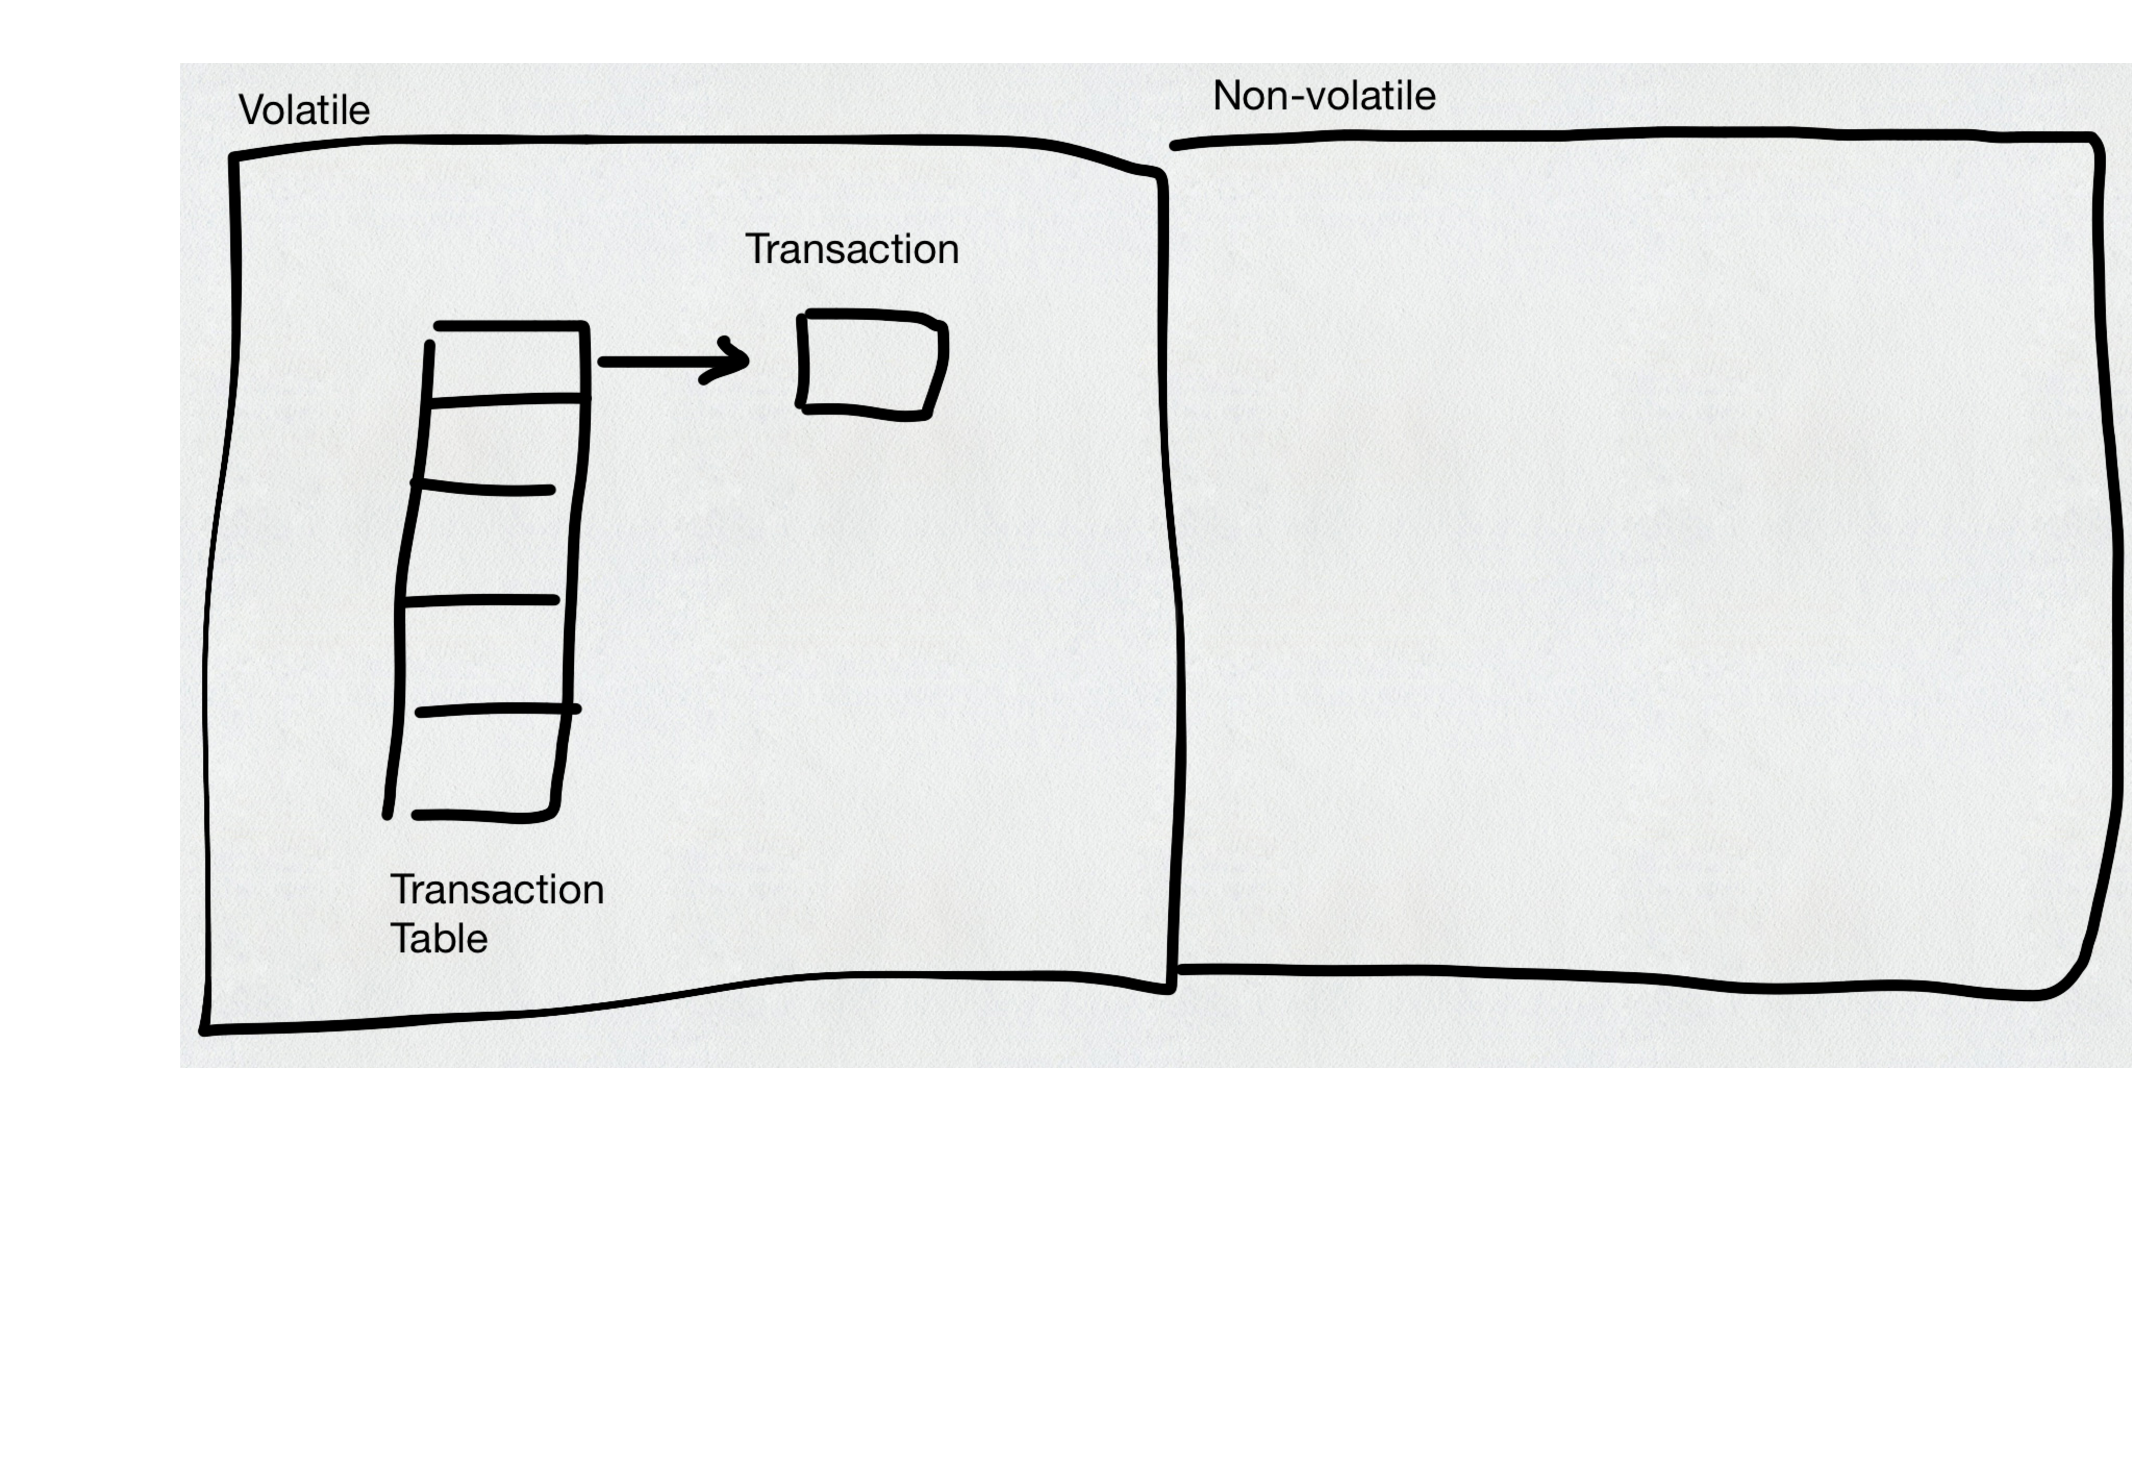
\includegraphics[width=\textwidth]{figures/drafts/concept-struct-volatile.pdf}
    \caption{}
    \label{fig:concept-struct-volatile}
\end{figure}

The non-volatile section stores all data that are durable across restarts. It
holds a control block, the index structure, and all data items mapped by the
index.

\paragraph{Control Block}

The control block is used to store a few essential metadata and for locating
the index after a restart. For that purpose, the control block is placed in a
fixed position of the KVS' non-volatile region. Possible locations are the front
or rear end of the memory region. The index can be found by storing an offset or
pointer. Either way, the underlying system must provide a way to reuse or
recover a previous memory mapping, so both location methods are sufficient.

\paragraph{Index}

The index implements the actual KVS paradigm by mapping keys to individual data
items. Note that, due to MVCC, instead of mapping concrete data items, each key
maps to a history of versions of its associated item. It is the core data
structure of a KVS and accessed by all transactions concurrently. As such, the
index is a strong contention point that is also very critical for the
performance of the KVS. For that reason, selecting a suitable data structure is
crucial. The domain analysis in Chapter \ref{ch:kvs-nvram} shows that many, if
not most, KVS rely on hash tables. Reasons are amortized constant access,
well-known array-like allocation schemes, and comparably low complexity. B-trees
or radix trees, on the other hand, are slower and optimized for disk storage
which was shown to be inappropriate for NVRAM. Therefore, this work opts for an
index based on a hash table.

Operations on the index include adding, retrieving, and removing a key-value
pair. To prevent inconsistencies through race conditions, access must be
mutually exclusive. While locking can quickly become a bottleneck in
read-dominated scenarios, non-blocking data structures are generally slower and
more complex. The actual hashing method is an implementation detail.

\paragraph{Histories}

The index maps each key to a chain of versions of a data item. Before an
operation on an item can begin, the MVCC algorithm has to determine which
version of the item is visible to the requesting transaction. As a result,
histories may be iterated frequently. Also multiple transactions may access the
same history at a time, so there may be overlapping accesses. However,
transactions never remove and only add new versions at the back of the history.
Therefore, contention may be high but mostly read-only. In order to account for
these characteristics, an array-like data structure may be the most appropriate
choice as opposed to a list. Consecutive access in arrays is less likely to
cause page faults and can benefit from hardware prefetching. Also arrays have
simpler allocation patterns compared to lists. Problems arise with garbage
collection which could perform random-access modifications to the history. Since
garbage collection would break the scope of this work, it is assumed to be
absent or as non-invasive as possible.

% \todo[inline]{insert figure here (WITH details on durable section)}

\begin{figure}[!ht]
    \centering
    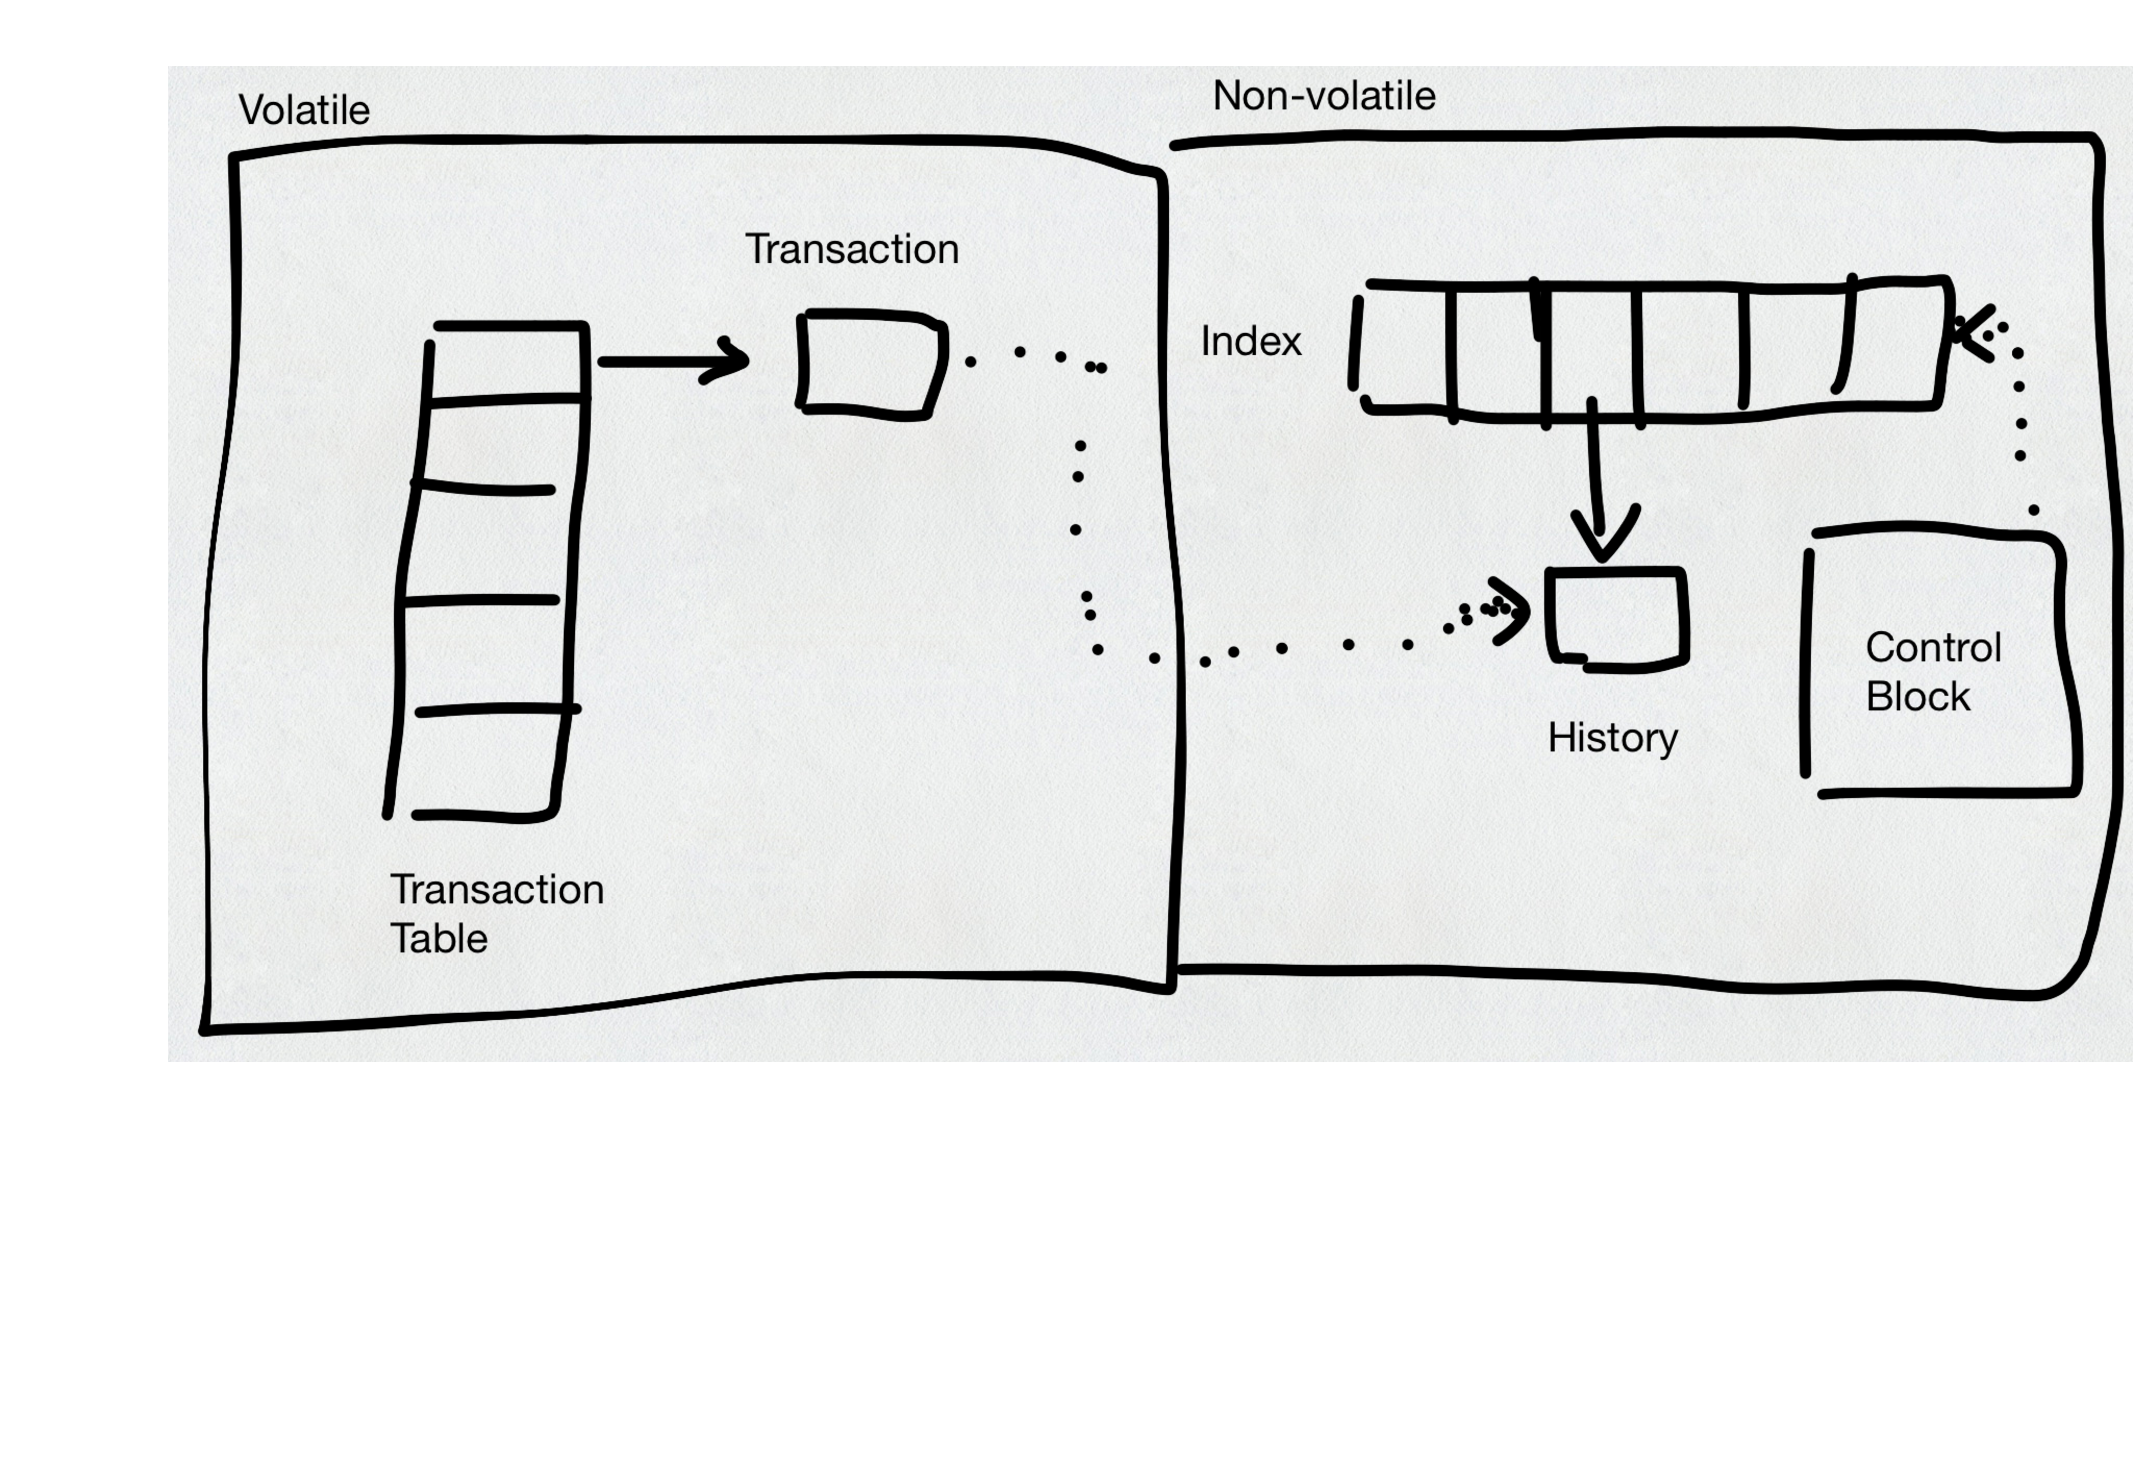
\includegraphics[width=\textwidth]{figures/drafts/concept-struct-complete.pdf}
    \caption{}
    \label{fig:concept-struct-complete}
\end{figure}
